\documentclass{article}

%%%%%%%%%%%%%%%%%%%%%%%%%
% Packages & Macros
%%%%%%%%%%%%%%%%%%%%%%%%%

% For including graphics
\usepackage{graphicx}

% For title page
\usepackage{datetime}
\newdateformat{monthyeardate}{\monthname[\THEMONTH] \THEYEAR}

% For supporting linking
\usepackage{hyperref}
\hypersetup{colorlinks,urlcolor=blue,linkcolor=blue,anchorcolor=blue,citecolor=blue}

% For table colouring (in command line tables)
\usepackage{colortbl}

%%%%%%%%%%%%%%%%%%%%%%%%%
% Tool-Specific Macros
%%%%%%%%%%%%%%%%%%%%%%%%%
\usepackage{xspace}

\newcommand{\args}[1] {\textit{#1}}
\newcommand{\cmd}[1] {\texttt{#1}}     % Use for command window commands, e.g., \cmd{svn up}
\newcommand{\block}[1] {\textsf{#1}}   % Use for Simulink block names, e.g., \cmd{Subsystem1}
\newcommand{\signal}[1] {\textsf{#1}}   % Use for Simulink block names, e.g., \cmd{Subsystem1}
\newcommand{\ring}[1] {\textsf{#1}} 	 % Use for files names and paths
\newcommand{\keyword}[1] {\texttt{#1}} % Use for keywords of programming languages, e.g., \keyword{while}
\newcommand{\file}[1] {\texttt{#1}} 	 % Use for files names and paths
\newcommand{\param}[1] {\textsf{#1}}   % Use for block parameter names, e.g., \param{BlockType}

% Matlab Products
\newcommand{\matlab}{\textsc{Matlab}\@\xspace}
\newcommand{\Matlab}{\textsc{Matlab}\@\xspace}
\newcommand{\Simulink}{Simulink\@\xspace}
\newcommand{\simulink}{Simulink\@\xspace}
\newcommand{\SDV}{Simulink Design Verifier\@\xspace}
\newcommand{\mpath}{\Matlab search path\@\xspace}

% Block Names (not BlockType)
\newcommand{\ds}{\block{Data Store}\@\xspace}
\newcommand{\DSM}{\block{Data Store Memory}\@\xspace}
\newcommand{\DSR}{\block{Data Store Read}\@\xspace}
\newcommand{\DSW}{\block{Data Store Write}\@\xspace}
\newcommand{\DSRW}{\block{Data Store Read/Write}\@\xspace}
\newcommand{\DSMRW}{\block{Data Store Memory/Read/Write}\@\xspace}

\newcommand{\goto}{\block{Goto}\@\xspace}
\newcommand{\from}{\block{From}\@\xspace}

\newcommand{\inport}{\block{Inport}\@\xspace}
\newcommand{\outport}{\block{Outport}\@\xspace}
\newcommand{\constant}{\block{Constant}\@\xspace}
\newcommand{\ground}{\block{Ground}\@\xspace}
\newcommand{\subsystem}{\block{Subsystem}\@\xspace}

\newcommand{\logic}{\block{Logical Operator}\@\xspace}
\newcommand{\relational}{\block{Relational Operator}\@\xspace}
\newcommand{\ifblk}{\block{If}\@\xspace}
\newcommand{\switch}{\block{Switch}\@\xspace}
\newcommand{\merge}{\block{Merge}\@\xspace}

\newcommand{\docblock}{\block{DocBlock}\@\xspace}

\newcommand{\simfunc}{\block{Simulink Function}\@\xspace}
\newcommand{\simfunccaller}{\block{Function Caller}\@\xspace}

\newcommand{\toworkspace}{\block{To Workspace}\@\xspace}
\newcommand{\fromworkspace}{\block{From Workspace}\@\xspace}

\newcommand{\tofile}{\block{To File}\@\xspace}
\newcommand{\fromfile}{\block{From File}\@\xspace}

\newcommand{\fromspreadsheet}{\block{From Spreadsheet}\@\xspace}

\newcommand{\modelref}{\block{Model Reference}\@\xspace}
\newcommand{\library}{\block{Library}\@\xspace}
\newcommand{\librarylink}{\block{Library Link}\@\xspace}

% Commonly used parameters
\newcommand{\AND}{\param{AND}\@\xspace}
\newcommand{\OR}{\param{OR}\@\xspace}
\newcommand{\NOT}{\param{NOT}\@\xspace}
\newcommand{\NOR}{\param{NOR}\@\xspace}
\newcommand{\NAND}{\param{NAND}\@\xspace}
\newcommand{\XOR}{\param{XOR}\@\xspace}
\newcommand{\NXOR}{\param{NXOR}\@\xspace}

% Common Abbreviations
% Example
\newcommand{\eg}{\textrm{e.g.,}\@\xspace}

% That Is To Say
\newcommand{\ie}{\textrm{i.e.,}\@\xspace}

% And So On
\newcommand{\etc}{\textrm{etc.}\@\xspace}

% And Others
\newcommand{\etal}{\textrm{et al.}\@\xspace}

% With Respect To
\newcommand{\wrt}{\textrm{w.r.t.}\@\xspace}

% Vice Versa
\newcommand{\vrsa}{\textrm{vice versa}\@\xspace}

% Symbols
\usepackage{amssymb}
\newcommand{\checkbox}{\makebox[0pt][l]{$\square$}\raisebox{.15ex}{\hspace{0.1em}$\checkmark$}}%
\newcommand{\uncheckbox}{$\square$~}%


\newcommand{\ToolName}{Reach/Coreach\@\xspace}
\newcommand{\Reach}{reach\@\xspace}
\newcommand{\Coreach}{coreach\@\xspace}

\newcommand{\menu}[1]{%
	\ifthenelse{\equal{#1}{1}}{Reach From Selected}{}%
	\ifthenelse{\equal{#1}{2}}{Coreach From Selected}{}%
	\ifthenelse{\equal{#1}{3}}{Reach/Coreach From Selected}{}%
	\ifthenelse{\equal{#1}{4}}{Clear Reach/Coreach}{}%
	\ifthenelse{\equal{#1}{5}}{Slice}{}%
	\ifthenelse{\equal{#1}{6}}{Set Colour}{}%
	\ifthenelse{\equal{#1}{7}}{Reach From Model Diff}{}%
	\ifthenelse{\equal{#1}{8}}{Coreach From Model Diff}{}%
}

\newcommand{\func}[1]{%
	\ifthenelse{\equal{#1}{1}}{ReachCoreach}{}%
	\ifthenelse{\equal{#1}{2}}{reachAll}{}%
	\ifthenelse{\equal{#1}{3}}{coreachAll}{}%
	\ifthenelse{\equal{#1}{4}}{clear}{}%
	\ifthenelse{\equal{#1}{5}}{slice}{}%
	\ifthenelse{\equal{#1}{6}}{setColor}{}%
	\ifthenelse{\equal{#1}{7}}{Reach\_Diff}{}%
	\ifthenelse{\equal{#1}{8}}{Coreach\_Diff}{}%
}

\newcommand{\toolFolder}{\cmd{ReachCoreach}}
\newcommand{\demoName}{\cmd{ReachCoreachDemo}\@\xspace}

\newcommand{\FCA}{0} 	% Enable/disabled FCA-specific content	
\newcommand{\HowSetPath}{\ifthenelse{\equal{\FCA}{1}}{If it is not, go to \cmd{File~>~Set~Path...}, press \cmd{Add with Subfolders}, and select the \cmd{McMaster\_Tools} folder. Restart \matlab after doing so.}{}}

%%%%%%%%%%%%%%%%%%%%%%%%%
% Document
%%%%%%%%%%%%%%%%%%%%%%%%%

\title{\ToolName Tool}
\date{\monthyeardate\today}

\begin{document}

%%%%%%%%%%%%%%%%%%%%%%%%%%%%%%%%%%%%%%%%%%%%%%%%%%%%%%%%%%%%%%%%%%%
% Title Page
%%%%%%%%%%%%%%%%%%%%%%%%%%%%%%%%%%%%%%%%%%%%%%%%%%%%%%%%%%%%%%%%%%%
\maketitle
\vfill

\begin{figure}
	\centering
	
\includegraphics[]{../figs/McSCert_Logo.pdf} \\
	McMaster Centre for Software Certification (McSCert)
\end{figure}

\newpage

%%%%%%%%%%%%%%%%%%%%%%%%%%%%%%%%%%%%%%%%%%%%%%%%%%%%%%%%%%%%%%%%%%%
% Table of Contents
%%%%%%%%%%%%%%%%%%%%%%%%%%%%%%%%%%%%%%%%%%%%%%%%%%%%%%%%%%%%%%%%%%%
\tableofcontents
\newpage

%%%%%%%%%%%%%%%%%%%%%%%%%%%%%%%%%%%%%%%%%%%%%%%%%%%%%%%%%%%%%%%%%%%
% Introduction
%%%%%%%%%%%%%%%%%%%%%%%%%%%%%%%%%%%%%%%%%%%%%%%%%%%%%%%%%%%%%%%%%%%
\section{Introduction}

% Briefly, what is the tool?
The \ToolName Tool is used to trace and highlight data flow and control flow dependencies in Simulink models. Performing a \emph{reachability analysis}, or ``\emph{reach}", on a portion of the model will show the effects that it has on other parts of the model. A \emph{coreachability analysis}, or ``\emph{coreach}", does the opposite, by showing what a portion of the model is dependent on.

The tool has many uses:
\begin{itemize}

	\item The reachability and coreachability analyses effectively generate a dependency diagram of data and control flow in the model. This assists with model comprehension, and is also useful in identifying areas of the model where seemingly independent data flows have hidden dependencies.
	\item The tool supports impact analysis, because it identifies the parts of a model affected by a potential change of a given block or signal. Impact analysis can be of great value in indicating what effect a change in requirements or design can have on a system's design.
	\item The tool can be used to find unreachable parts of a model. When reachability analysis is performed on all of a model's inputs, unhighlighted blocks/signals represent unreachable parts of the model. 
	\item When the coreachability analysis is performed on all of a model's outputs, the unhighlighted blocks/signals are unnecessary in the sense that they have no (data or control) effect on the outputs of the model.
	\item The tool can isolate a model into smaller pieces for further analysis, by \emph{slicing} out the highlighted traces.
\end{itemize}

% Is there more information?
\subsection{More Information}
For more information on the tool and how it can be used in a model-based development with Simulink, please refer to the following papers:

\vspace{1em}
Vera Pantelic, Steven Postma, Mark Lawford, Monika Jaskolka, Bennett Mackenzie, Alexandre Korobkine, Marc Bender, Jeff Ong, Gordon Marks, Alan Wassyng, \href{https://link.springer.com/article/10.1007/s10009-017-0450-9}{``Software engineering practices and Simulink: bridging the gap,"} \textit{International Journal on Software Tools for Technology Transfer (STTT)}, 2017, 95--117.

\vspace{1em}
Vera Pantelic, Steven Postma, Mark Lawford, Alexandre Korobkine, Bennett Mackenzie, Jeff Ong, and Marc Bender, \href{http://www.cas.mcmaster.ca/~lawford/papers/MODELSWARD2015.pdf}{``A Toolset for Simulink: Improving Software Engineering Practices in Development with Simulink,"}\textit{Proceedings of 3rd International Conference on Model-Driven Engineering and Software Development (MODELSWARD 2015)}, SCITEPRESS, 2015, 50--61.

%%%%%%%%%%%%%%%%%%%%%%%%%%%%%%%%%%%%%%%%%%%%%%%%%%%%%%%%%%%%%%%%%%%
% How to Use the Tool
%%%%%%%%%%%%%%%%%%%%%%%%%%%%%%%%%%%%%%%%%%%%%%%%%%%%%%%%%%%%%%%%%%%
\section{How to Use the Tool}
This section describes what must be done to setup the tool, as well as how to use the tool.

%---------------------------------------
% What needs to be done before the tool can be used? 
% What needs to be done to a model in order for it to work on said model?
%---------------------------------------
\subsection{Prerequisites and Installation}

\begin{enumerate}
	\item Use \Matlab/\Simulink 2011b or newer.
	\item To install the tool,
	\begin{enumerate}
		\item from a \file{.zip} file --- unzip the contents into your desired location. Ensure the unzipped folder and subfolders are present in your \mpath, or add them if they are not present. Run \href{https://www.mathworks.com/help/simulink/ug/registering-customizations.html}{sl\_refresh\_customizations} to refresh the Context Menu. 
		\item from a \file{.mltbx} file --- simply open \Matlab and double-click on the file. Your \mpath should be automatically configured.
		\item from the files only --- add the folders and subfolders to your \mpath. Run \href{https://www.mathworks.com/help/simulink/ug/registering-customizations.html}{sl\_refresh\_customizations} to refresh the Context Menu.
	\end{enumerate}
	\begin{itemize}
		\item \textit{Note:} If running the command ``\cmd{which ReachCoreach}'' indicates that the script is not found, then the tool needs to be added to the \mpath.
		For information on adding files to the \mpath, please see the \href{https://www.mathworks.com/help/matlab/matlab_env/add-remove-or-reorder-folders-on-the-search-path.html}{MathWorks documentation}.
	\end{itemize}
	\item Ensure the Simulink-Utility folder is on your \mpath. This is a dependency for the tool to work correctly.
	\item Ensure your model is open and unlocked.
\end{enumerate}


%---------------------------------------
% How/when do you access the tool?
%---------------------------------------
\subsection{Getting Started}
Most features of the tool can be used via the Simulink Context Menu, which can be viewed by right-clicking in a model. The following options can be available in the \ToolName menu, depending on what is selected in the model. These options are shown in Figure~\ref{FIG:contextMenu}.
\begin{itemize}
	\item \emph{\menu{1}} -- Available at all times.
	\item \emph{\menu{2}} -- Available at all times.
	\item \emph{\menu{3}} -- Available at all times.
	\item \emph{\menu{4}} -- Available when a \Reach and/or \Coreach are present in the model.
	\item \emph{\menu{5}} -- Available when a \Reach and/or \Coreach are present in the model.
	\item \emph{\menu{6}} -- Available at all times.
\end{itemize}

The only features that cannot be used via the Simulink Context Menu are the model differencing versions of the \cmd{\menu{1}} and \cmd{\menu{2}} functionalities which are run via the command line, as described in Table ~\ref{tab:reach-diff} and Table ~\ref{tab:coreach-diff}.

\begin{figure}
	\centering
	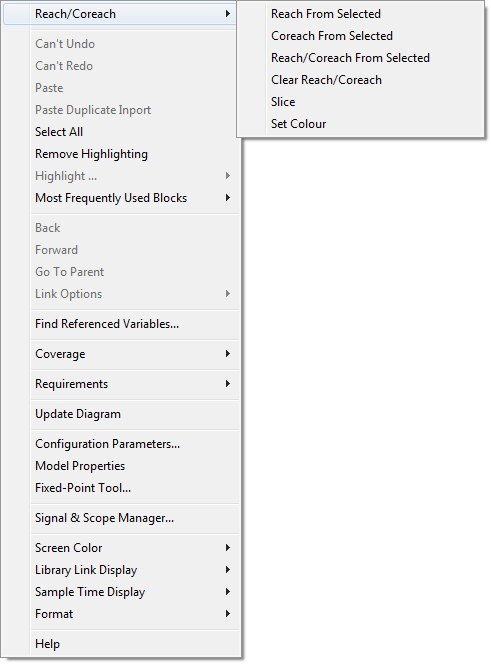
\includegraphics[width=0.7\textwidth]{../figs/ContextMenu}
	\caption{Simulink Context Menu with tool options visible.}
	\label{FIG:contextMenu}
\end{figure}

%---------------------------------------
% What are the main uses of the tool?
%---------------------------------------
\subsection{Functionality}
This section describes the tool functionality when being used from the Simulink Context Menu (Figure~\ref{FIG:contextMenu}).

\subsubsection*{\menu{1}}
Right-clicking on one or more blocks in the model and then selecting \cmd{\menu{1}} from the Context Menu will perform a reachability analysis, and highlight the blocks and signals which are affected by those selected blocks. The highlighting illustrates what parts of the model are dependent on the selected blocks, due to control flow or data flow.

\subsubsection*{\menu{2}}
Right-clicking on one or more blocks in the model and then selecting \cmd{\menu{2}} from the Context Menu will perform a coreachability analysis, and highlight the blocks and signals which affect those selected blocks. The highlighting illustrates what parts of the model the selected blocks depend on, due to control flow or data flow.

\subsubsection*{\menu{3}}
Right-clicking on one or more blocks in the model, and then selecting \cmd{\menu{3}} from the Context Menu will perform both reachability and coreachability analyses on the selected blocks. The highlighting illustrates, bidirectionally, what parts of the model either impact, or have an impact, on the selected blocks, due to control flow or data flow.

\subsubsection*{\menu{4}}
After a \Reach, \Coreach, or \Reach/\Coreach are performed on the model, this option will be enabled. Right-clicking anywhere in the model, and then selecting \cmd{\menu{4}} from the Context Menu will clear all highlighting in the model.

\subsubsection*{\menu{5}}
After a \Reach, \Coreach, or \Reach/\Coreach are performed on the model, this option will be enabled. Right-clicking anywhere in the model, and then selecting \cmd{\menu{5}} from the Context Menu will isolate the highlighted parts of the model by removing the non-highlighted blocks and lines.

\subsubsection*{\menu{6}}
Right-clicking anywhere in the model and then selecting \cmd{\menu{6}} from the Context Menu will display the user interface shown in Figure~\ref{FIG:gui}. The foreground (text and line) and background (block) highlight colours can be customized via the drop down menus, which provide the standard Matlab colours. Clicking \cmd{OK} will use the selected colours for all current and future highlighting in the model. The default colours are red (foreground) and yellow (background).

\begin{figure}
	\centering
	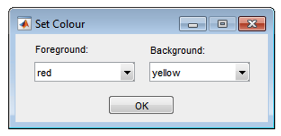
\includegraphics[width=0.6\textwidth]{../figs/GUI}
	\caption{Highlight colour selector interface.}
	\label{FIG:gui}
\end{figure}

%---------------------------------------
% What else does the tool do?
%---------------------------------------
\subsection{Errors and Warnings}
Any errors or warnings during tool use will be visible in the \matlab Command Window. Typically, errors will be shown when the model is locked or function parameters are incorrect.  

%%%%%%%%%%%%%%%%%%%%%%%%%%%%%%%%%%%%%%%%%%%%%%%%%%%%%%%%%%%%%%%%%%%
% Example
%%%%%%%%%%%%%%%%%%%%%%%%%%%%%%%%%%%%%%%%%%%%%%%%%%%%%%%%%%%%%%%%%%%
\section{Example}

Use the command \demoName in the Simulink command window to open the example model, shown in Figure~\ref{FIG:demo1}. This example has control and data flow pass through \block{Data Store}s, \block{If} and \block{If Action} subsystems, as well as a \block{Bus Creator} and \block{Bus Selector}. The following steps will demonstrate the various functionalities of the tool.

\begin{enumerate}
	\item Let us perform a reachability analysis to find all possible dependencies of the \block{Inport} block \block{In2}. To do this, right-click on the  \block{In2} block and select the \cmd{\menu{1}} option. The resulting model is shown in Figure~\ref{FIG:demo2}. Due to the fact that \block{In2} is used in the last two condition checks of the \block{If} block and its data flow is traced to \block{Outport} block \block{Out1}. Doing a reachability analysis on \block{In2} also shows clearly that it impacts the \DSM block \block{A}.
\end{enumerate}

\begin{figure}
	\centering
	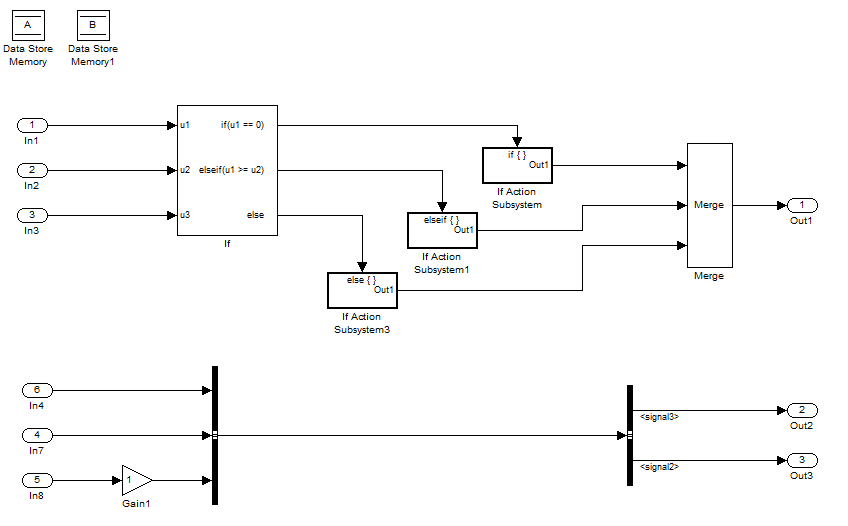
\includegraphics[width=0.9\textwidth]{../figs/Demo1}
	\caption{\ToolName demo model.}
	\label{FIG:demo1}
\end{figure}

\begin{enumerate}
	\item[2.] To clear the highlighting now present in the model due to the previous \Reach operation, right-click anywhere in the model and select the \cmd{\menu{4}} option. This will revert the model's appearance to that of Figure~\ref{FIG:demo1}.
\end{enumerate}

\begin{figure}[ht!]
	\centering
	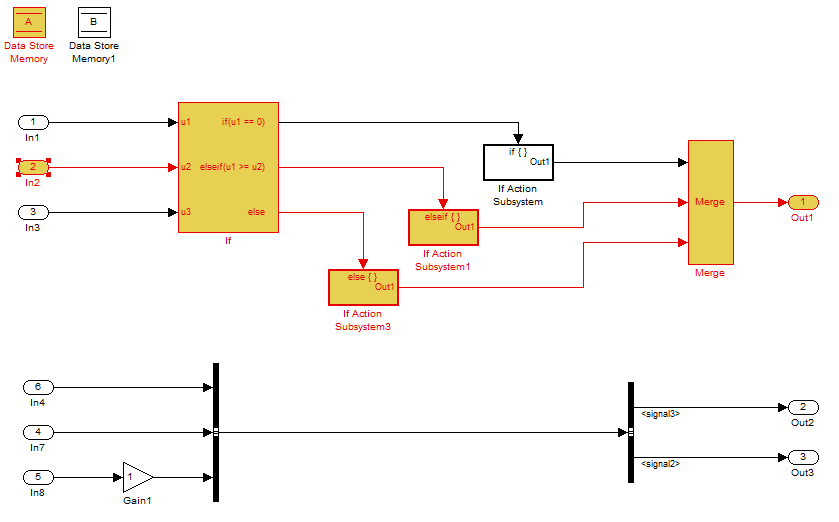
\includegraphics[width=0.9\textwidth]{../figs/Demo2}
	\caption{Resulting model after \cmd{Reach From Selected} operation.}
	\label{FIG:demo2}
\end{figure}

\begin{enumerate}
	\item[3.]  Let us perform a coreachability analysis to find all the parts of the model which the \block{Outport} blocks \block{Out2} and \block{Out3} are dependent on. To do this, select both blocks, right-click on them, and select the \cmd{\menu{2}} option. The resulting model is shown in Figure~\ref{FIG:demo3}. Blocks \block{Out2} and \block{Out3} are dependent on the \block{Inport} block \block{In7} and \block{In8} only, and it is interesting to note that \block{In6} has no impact in the model.
\end{enumerate}

\begin{figure}[ht!]
	\centering
	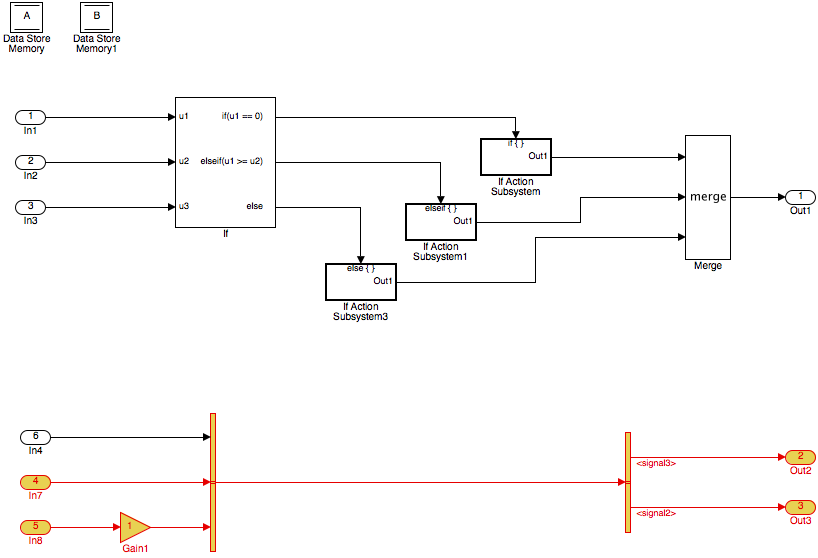
\includegraphics[width=0.9\textwidth]{../figs/Demo3}
	\caption{Resulting model after \cmd{Coreach From Selected} operation.}
	\label{FIG:demo3}
\end{figure}

\begin{enumerate}
	\item[4.] We can isolate the coreachability analysis by performing a slice. To do so, right-click anywhere in the model and select the \cmd{\menu{5}} option. All blocks and signals which are not highlighted will be deleted from the model. The resulting model is shown in Figure~\ref{FIG:demo4}.
\end{enumerate}

\begin{figure}[ht!]
	\centering
	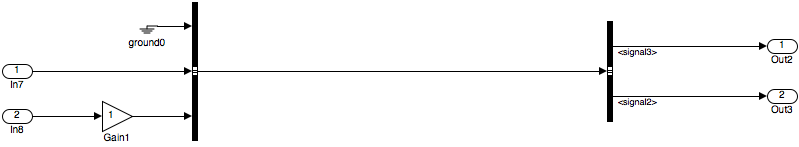
\includegraphics[width=0.9\textwidth]{../figs/Demo4}
	\caption{Resulting model after \cmd{Slice} operation.}
	\label{FIG:demo4}
\end{figure}

\begin{enumerate}
	\item[5.] Let us now perform a \Reach/\Coreach in the model. First, reopen the demo model, so as to start from new. Right-click on \DSM \block{B},  and select the \cmd{\menu{3}} option.  The resulting model is shown in Figure~\ref{FIG:demo5}. By doing both a reachability and coreachability analysis on this block, we can see the total impact that this block has on the model. In this case, no other blocks or signals are highlighted, meaning that this block has no purpose in the model. It is not used by anything, nor does it perform any operation itself. This block can be considered ``dead code", and should be removed from the design.
\end{enumerate}

\begin{figure}[ht!]
	\centering
	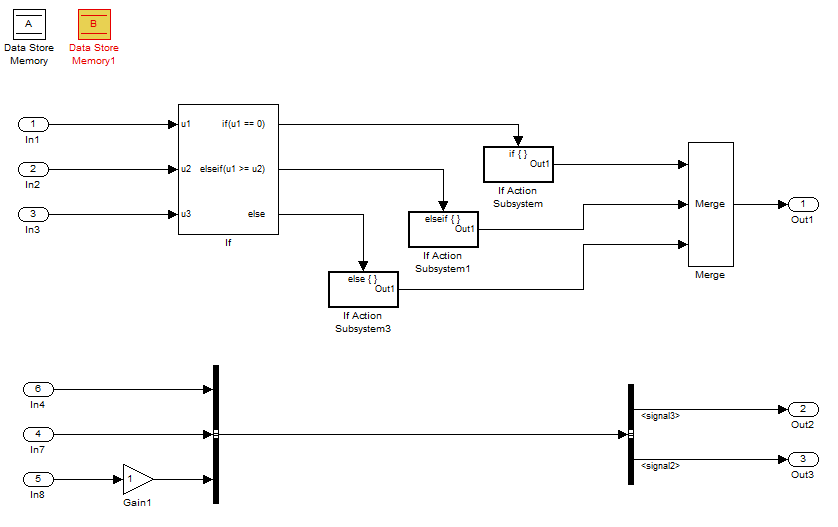
\includegraphics[width=0.9\textwidth]{../figs/Demo5}
	\caption{Resulting model after \cmd{Reach/Coreach} operation.}
	\label{FIG:demo5}
\end{figure}

%%%%%%%%%%%%%%%%%%%%%%%%%%%%%%%%%%%%%%%%%%%%%%%%%%%%%%%%%%%%%%%%%%%
% Matlab Commands
%%%%%%%%%%%%%%%%%%%%%%%%%%%%%%%%%%%%%%%%%%%%%%%%%%%%%%%%%%%%%%%%%%%
\newpage
\section{Matlab Commands}

The tool can also be used via the \matlab command line, with the following classes and functions.

%%---------------------------------------
%% Command 1
%%---------------------------------------
%\begin{center}
%	\begin{tabular}{| >{\columncolor[gray]{0.9}}l | p{8.5cm} |} \hline
%		Function 		& \cmd{\func{1}} \\ \hline
%		Syntax			& \cmd{\func{1}}(\args{model, dontMove}) \\ \hline
%		Description		& Rescopes all \DSM blocks except for those listed in \args{dontMove}. \\ \hline
%		Input Arguments	& \args{model}: The Simulink model name (or top-level system name) of the model on which to perform the rescoping operation. \newline
%						  \args{dontMove}: A cell array of \DSM path names which are not to be moved. \\ \hline	
%	\end{tabular}
%\end{center}
%
%\paragraph{Example:} The following command moves all \DSM blocks in the open/loaded model \demoName to their proper level in the hierarchy such that \DSRW references remain within scope. The resulting model is shown as Figure~\ref{FIG:demo2}.
%
%\begin{center}
%	\cmd{\func{1}~(`\demoName', \{\})}
%\end{center}

%---------------------------------------
% Command 1
%---------------------------------------
\begin{table}[!hp]
	\centering
	\caption{ReachCoreach function description.}
	\begin{tabular}{| >{\columncolor[gray]{0.9}}l | p{8.5cm} |} \hline
		Function 		& \cmd{\func{1}} \\ \hline
		Syntax			& \cmd{obj = \func{1}}(\args{modelName}) \\ \hline
		Description		& Create a new  ReachCoreach object for \args{model}. \\ \hline
		Inputs	& \args{modelName}: The Simulink model name (or top-level system name) of the model on which to perform \Reach/\Coreach operations. \\ \hline
		Outputs			& \args{obj}: ReachCoreach object. \\ \hline
	\end{tabular}
\end{table}


%---------------------------------------
% Command 2
%---------------------------------------
\begin{table}[!hp]
	\centering
	\caption{reachAll function description.}
	\begin{tabular}{| >{\columncolor[gray]{0.9}}l | p{8.5cm} |} \hline
		Function 		& \cmd{\func{2}} \\ \hline
		Syntax			& \cmd{obj.\func{2}}(\args{blocks, lines}) \\ \hline
		Description		& Perform a reachability analysis starting from \args{blocks}. \\ \hline
		Inputs	& \args{blocks}: A cell array of block path names from which to start the \Reach operation. \newline 
		                  \args{lines}: An array of handles representing signal lines from which to start the \Reach operation. \\ \hline
		Outputs			& N/A \\ \hline
	\end{tabular}
\end{table}

%---------------------------------------
% Command 3
%---------------------------------------
\begin{table}[!hp]
	\centering
	\caption{coreachAll function description.}
	\begin{tabular}{| >{\columncolor[gray]{0.9}}l | p{8.5cm} |} \hline
		Function 		& \cmd{\func{3}} \\ \hline
		Syntax			& \cmd{obj.\func{3}}(\args{blocks, lines}) \\ \hline
		Description		& Perform a coreachability analysis starting from \args{blocks}. \\ \hline
		Inputs	& \args{blocks}: A cell array of block path names from which to start the \Coreach operation. \newline
		                  \args{lines}: An array of handles representing signal lines from which to start the \Coreach operation. \\ \hline
		Outputs			& N/A \\ \hline
	\end{tabular}
\end{table}

%---------------------------------------
% Command 4
%---------------------------------------
\begin{table}[!hp]
	\centering
	\caption{clear function description.}
	\begin{tabular}{| >{\columncolor[gray]{0.9}}l | p{8.5cm} |} \hline
		Function 		& \cmd{\func{4}} \\ \hline
		Syntax			& \cmd{obj.\func{4}}() \\ \hline
		Description		& Clear any \Reach or \Coreach highlighting. \\ \hline
		Inputs			& N/A \\ \hline
		Outputs			& N/A \\ \hline
	\end{tabular}
\end{table}

%---------------------------------------
% Command 5
%---------------------------------------
\begin{table}[!hp]
	\centering
	\caption{slice function description.}
	\begin{tabular}{| >{\columncolor[gray]{0.9}}l | p{8.5cm} |} \hline
		Function 		& \cmd{\func{5}} \\ \hline
		Syntax			& \cmd{obj.\func{5}}() \\ \hline
		Description		& Isolate the \Reach/\Coreach blocks by removing unhighlighted blocks. \\ \hline
		Inputs	& N/A \\ \hline	
		Outputs			& N/A \\ \hline
	\end{tabular}
\end{table}

%---------------------------------------
% Command 6
%---------------------------------------
\begin{table}[!hp]
	\centering
	\caption{setColor function description.}
	\begin{tabular}{| >{\columncolor[gray]{0.9}}l | p{8.5cm} |} \hline
		Function 		& \cmd{\func{6}} \\ \hline
		Syntax			& \cmd{obj.\func{6}}(\args{foregroundColor}, \args{backgroundColor}) \\ \hline
		Description		& Set the color of the \Reach/\Coreach highlighting. \\ \hline
		Inputs		& \args{foregroundColor}: A Matlab color. \newline
						  	\args{backgroundColor}: A Matlab color. \\ \hline
		Outputs		& N/A \\ \hline
	\end{tabular}
\end{table}

%---------------------------------------
% Command 7
%---------------------------------------
\begin{table}[!hp]
	\centering
	\caption{Reach\_Diff function description.}
	\label{tab:reach-diff}
	\begin{tabular}{| >{\columncolor[gray]{0.9}}l | p{10.5cm} |} \hline
		Function 		& \cmd{\func{7}} \\ \hline
		Syntax			& [rObjs1, rObjs2] = \cmd{\func{7}}(\args{model1, model2, highlight})\\ \hline
		Description		& Identify objects in \args{model1} and \args{model2} that were added/deleted/modified between the two versions, 
			then perform a reachability analysis in each model starting from the identified objects. \\ \hline
		Inputs			& 
		\args{model1}: A char array naming a model. \newline
		\args{model2}: A char array naming a different version of the model given by \args{model1} (this version can be newer or older). \newline
		\args{highlight}: Set as 1 to highlight impacts yellow within the models and to highlight the differences dark green; set as 0 for no highlighting. (Optional. Default is 1) \\ \hline
		Outputs 		& 
		\args{rObjs1}: Array of Simulink block and line handles that were reached in \args{model1} \newline
		\args{rObjs2}: Array of Simulink block and line handles that were reached in \args{model2}. \\ \hline
	\end{tabular}
\end{table}

%---------------------------------------
% Command 8
%---------------------------------------
\begin{table}[!hp]
	\centering
	\caption{Coreach\_Diff function description.}
	\label{tab:coreach-diff}
	\begin{tabular}{| >{\columncolor[gray]{0.9}}l | p{10.5cm} |} \hline
		Function 		& \cmd{\func{8}} \\ \hline
		Syntax			& [cObjs1, cObjs2] = \cmd{\func{8}}(\args{model1, model2, highlight}) \\ \hline
		Description		& Identify objects in \args{model1} and \args{model2} that were added/deleted/modified between the two versions, 
		then perform a coreachability analysis in each model starting from the identified objects. \\ \hline
		Inputs			& 
		\args{model1}: A char array naming a model. \newline
		\args{model2}: A char array naming a different version of the model given by \args{model1} (this version can be newer or older). \newline
		\args{highlight}: Set as 1 to highlight impacts yellow within the models and to highlight the differences dark green; set as 0 for no highlighting. (Optional. Default is 1) \\ \hline
		Outputs 		& 
		\args{cObjs1}: Array of Simulink block and line handles that were coreached in \args{model1}. \newline
		\args{cObjs2}: Array of Simulink block and line handles that were coreached in \args{model2}. \\ \hline
	\end{tabular}
\end{table}

%%%%%%%%%%%%%%%%%%%%%%%%%%%%%%%%%%%%%%%%%%%%%%%%%%%%%%%%%%%%%%%%%%%
% Example
%%%%%%%%%%%%%%%%%%%%%%%%%%%%%%%%%%%%%%%%%%%%%%%%%%%%%%%%%%%%%%%%%%%

\vspace{2em}

\paragraph{Example:} The following commands perform the same operations as described previously for the \demoName example, however via the Matlab command line.

\begin{enumerate}
	\item \cmd{r = \func{1}(`\demoName')} 			
	\item \cmd{r.\func{2}(\{`\demoName/In2'\})}			
	\item \cmd{r.\func{4}()}								
	\item \cmd{r.\func{3}(\{`\demoName/Out2',`\demoName/Out3'\})}	
	\item \cmd{r.\func{5}()}								
\end{enumerate}

\end{document}